\documentclass{article}

\usepackage{color}
\usepackage{graphicx}
\usepackage{amsmath}
\usepackage{geometry}
\geometry{left=2.54cm,right=2.54cm,top=2.54cm,bottom=2.54cm}
\begin{document}

\vspace*{0.25cm}

\hrulefill

\thispagestyle{empty}

\begin{center}
\begin{large}
\sc{UM--SJTU Joint Institute \vspace{0.3em} \\ Introduction to Operating Systems \\(VE482)}
\end{large}

\hrulefill

\vspace*{5cm}
\begin{Large}
\sc{{Laboratory Report}}
\end{Large}

\vspace{2em}

\begin{large}
\sc{{Lab 1
\vspace{0.5em}

}}
\end{large}
\end{center}


\vfill

\begin{table}[h!]
\flushleft
\begin{tabular}{lll}
Name: Ji Xingyou \hspace*{2em}&
ID: 515370910197\hspace*{2em}
\\

Date: 15 September 2017

\end{tabular}
\end{table}

\hfill
\begin{tiny}
[rev. 2.0]
\end{tiny}
\newpage
\section{Answer the following questions:}
\begin{itemize}
	\item \textbf{Where is the CPU hidden, and why?}\\
	The CPU is hidden under the radiator.\\
	The CPU works at a high power so that it emits lots of heat. A radiator is thus needed to cool the CPU down.
	The exact location is shown in figure 1.
	\begin{figure}[h!]
	\begin{center}
	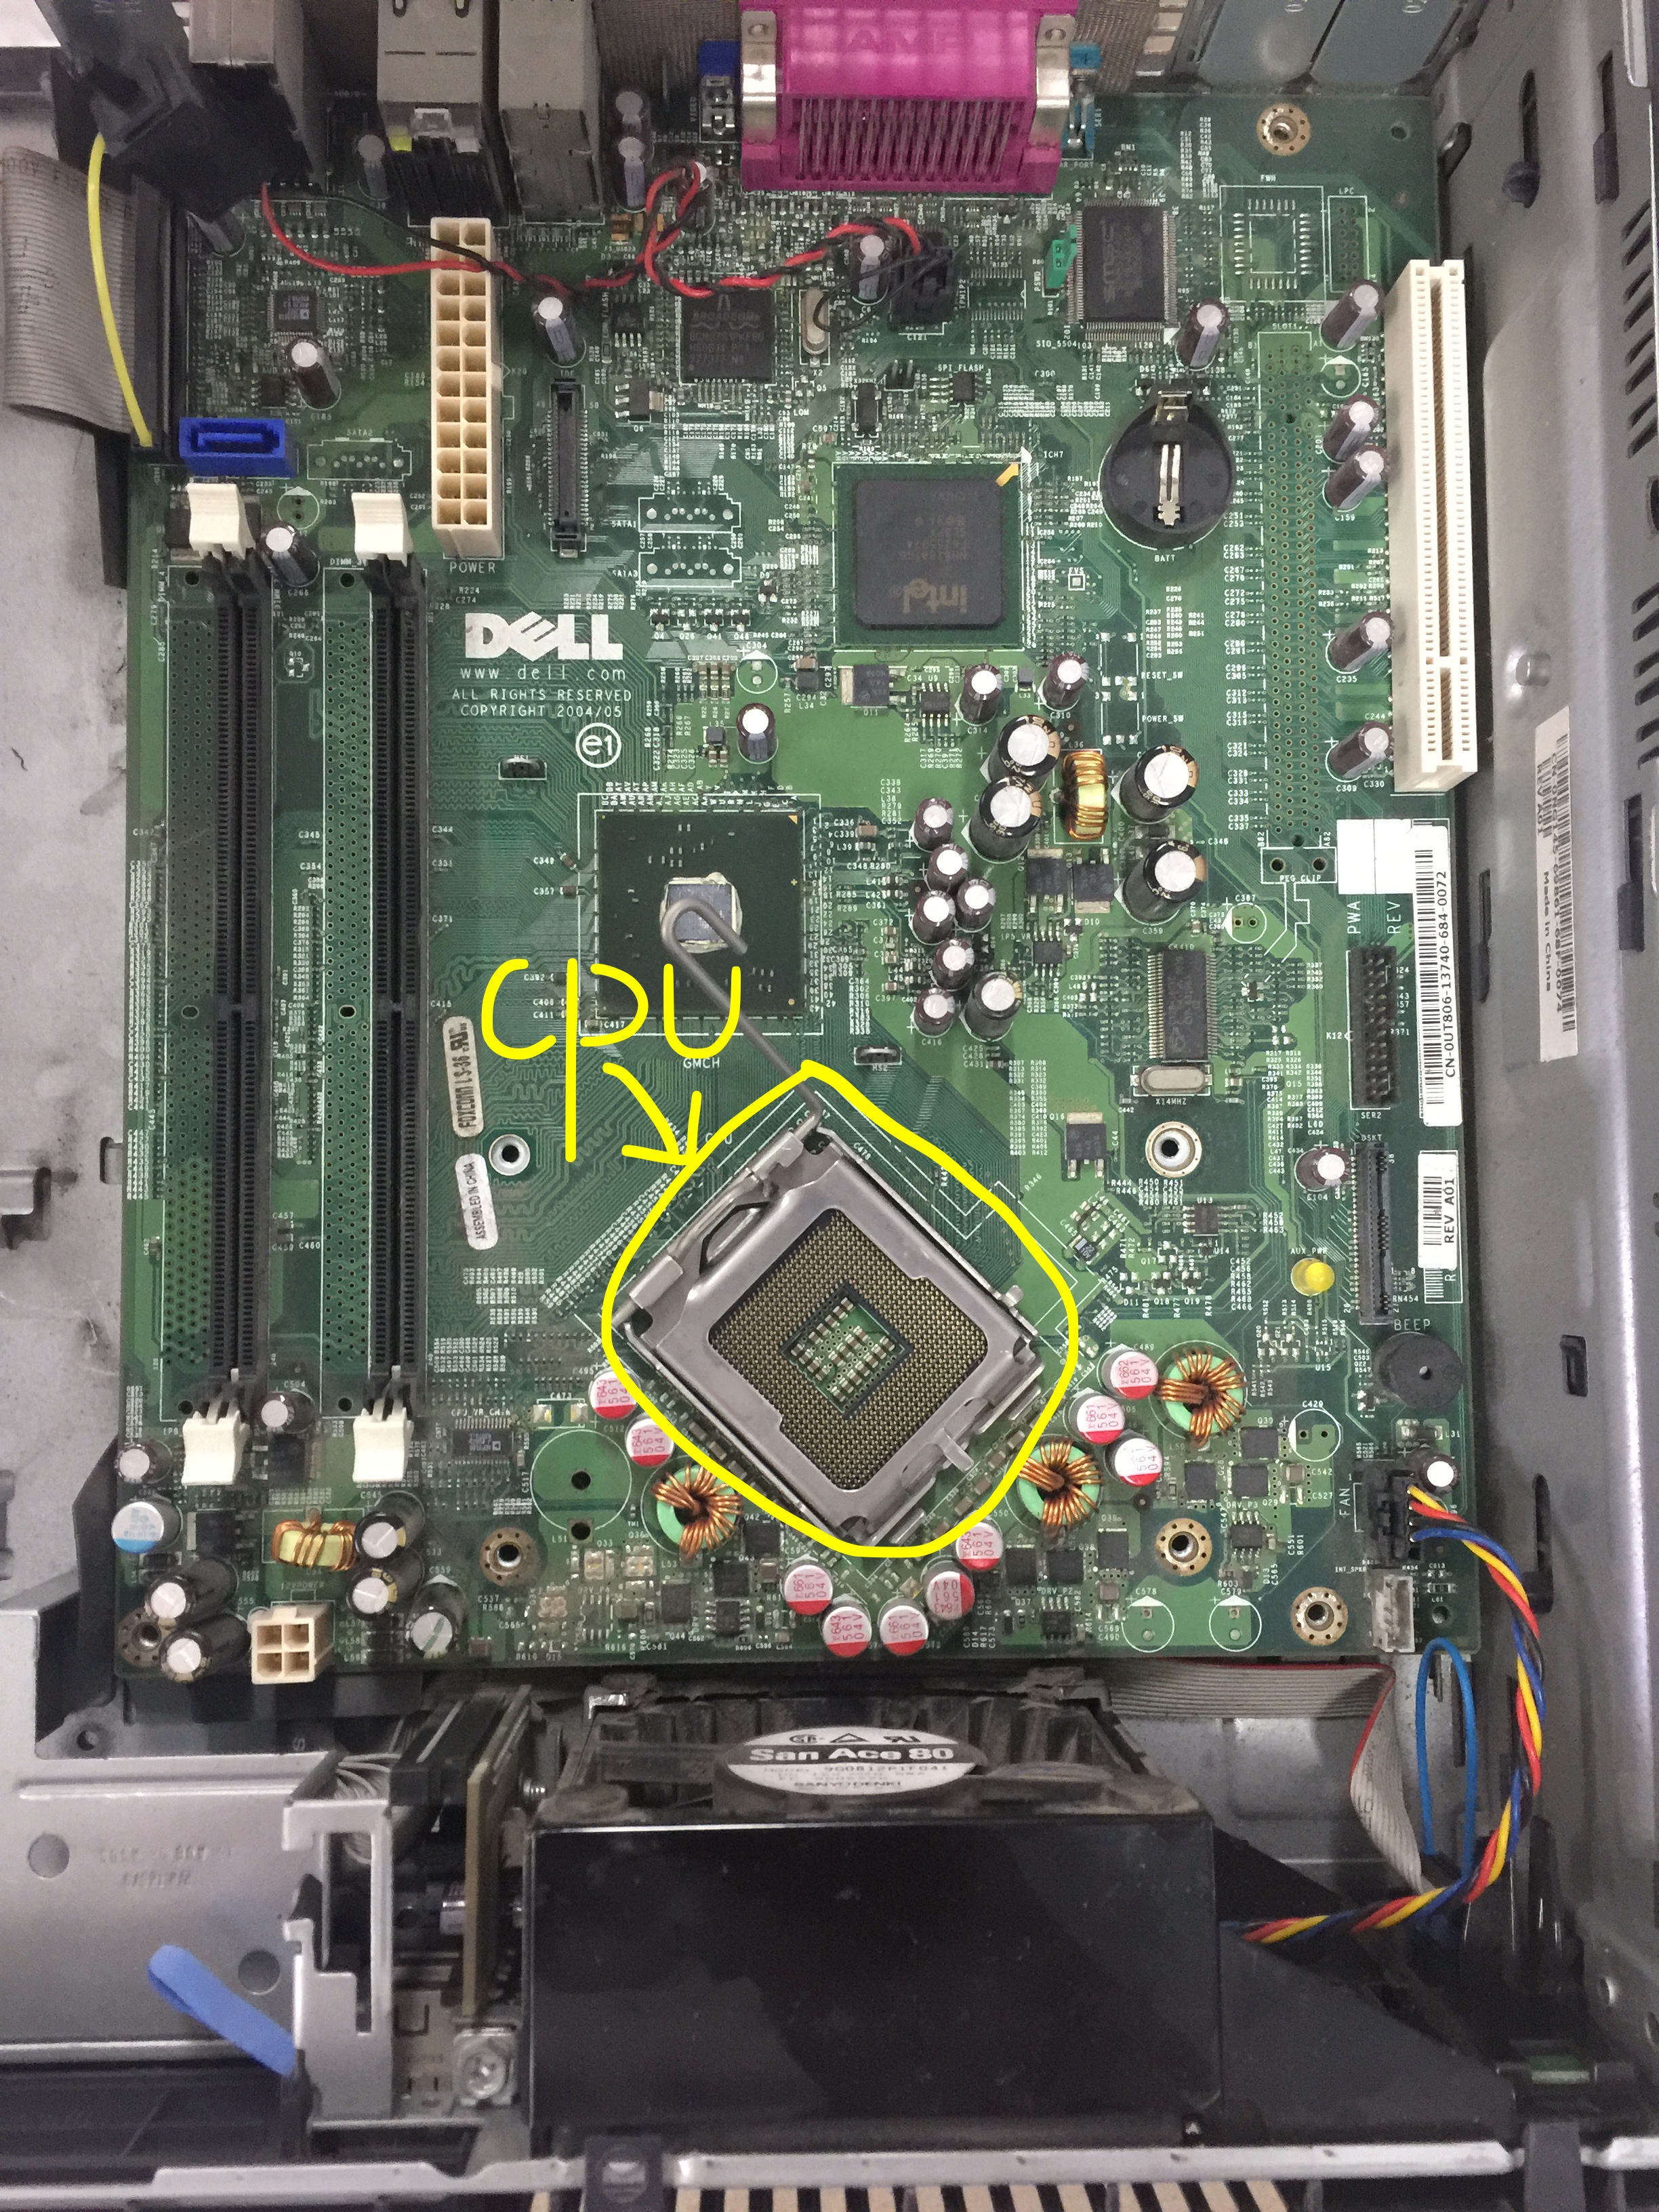
\includegraphics[scale=0.06]{CPU.jpg}
	\caption{The location of CPU on the mother board.}
	\end{center}
	\end{figure}
	\item \textbf{What are the North and South bridges?}\\
	North bridge is responsible for the communication with the CPU, and other tasks that require the highest performance. Therefore, north bridge is placed the nearest to the CPU.\\
	South bridge is responsible for input and output control, and other tasks that only need low speed.
	The location of north bridge and south bridge is shown in figure 2.
	\begin{figure}[h!]
	\begin{center}
	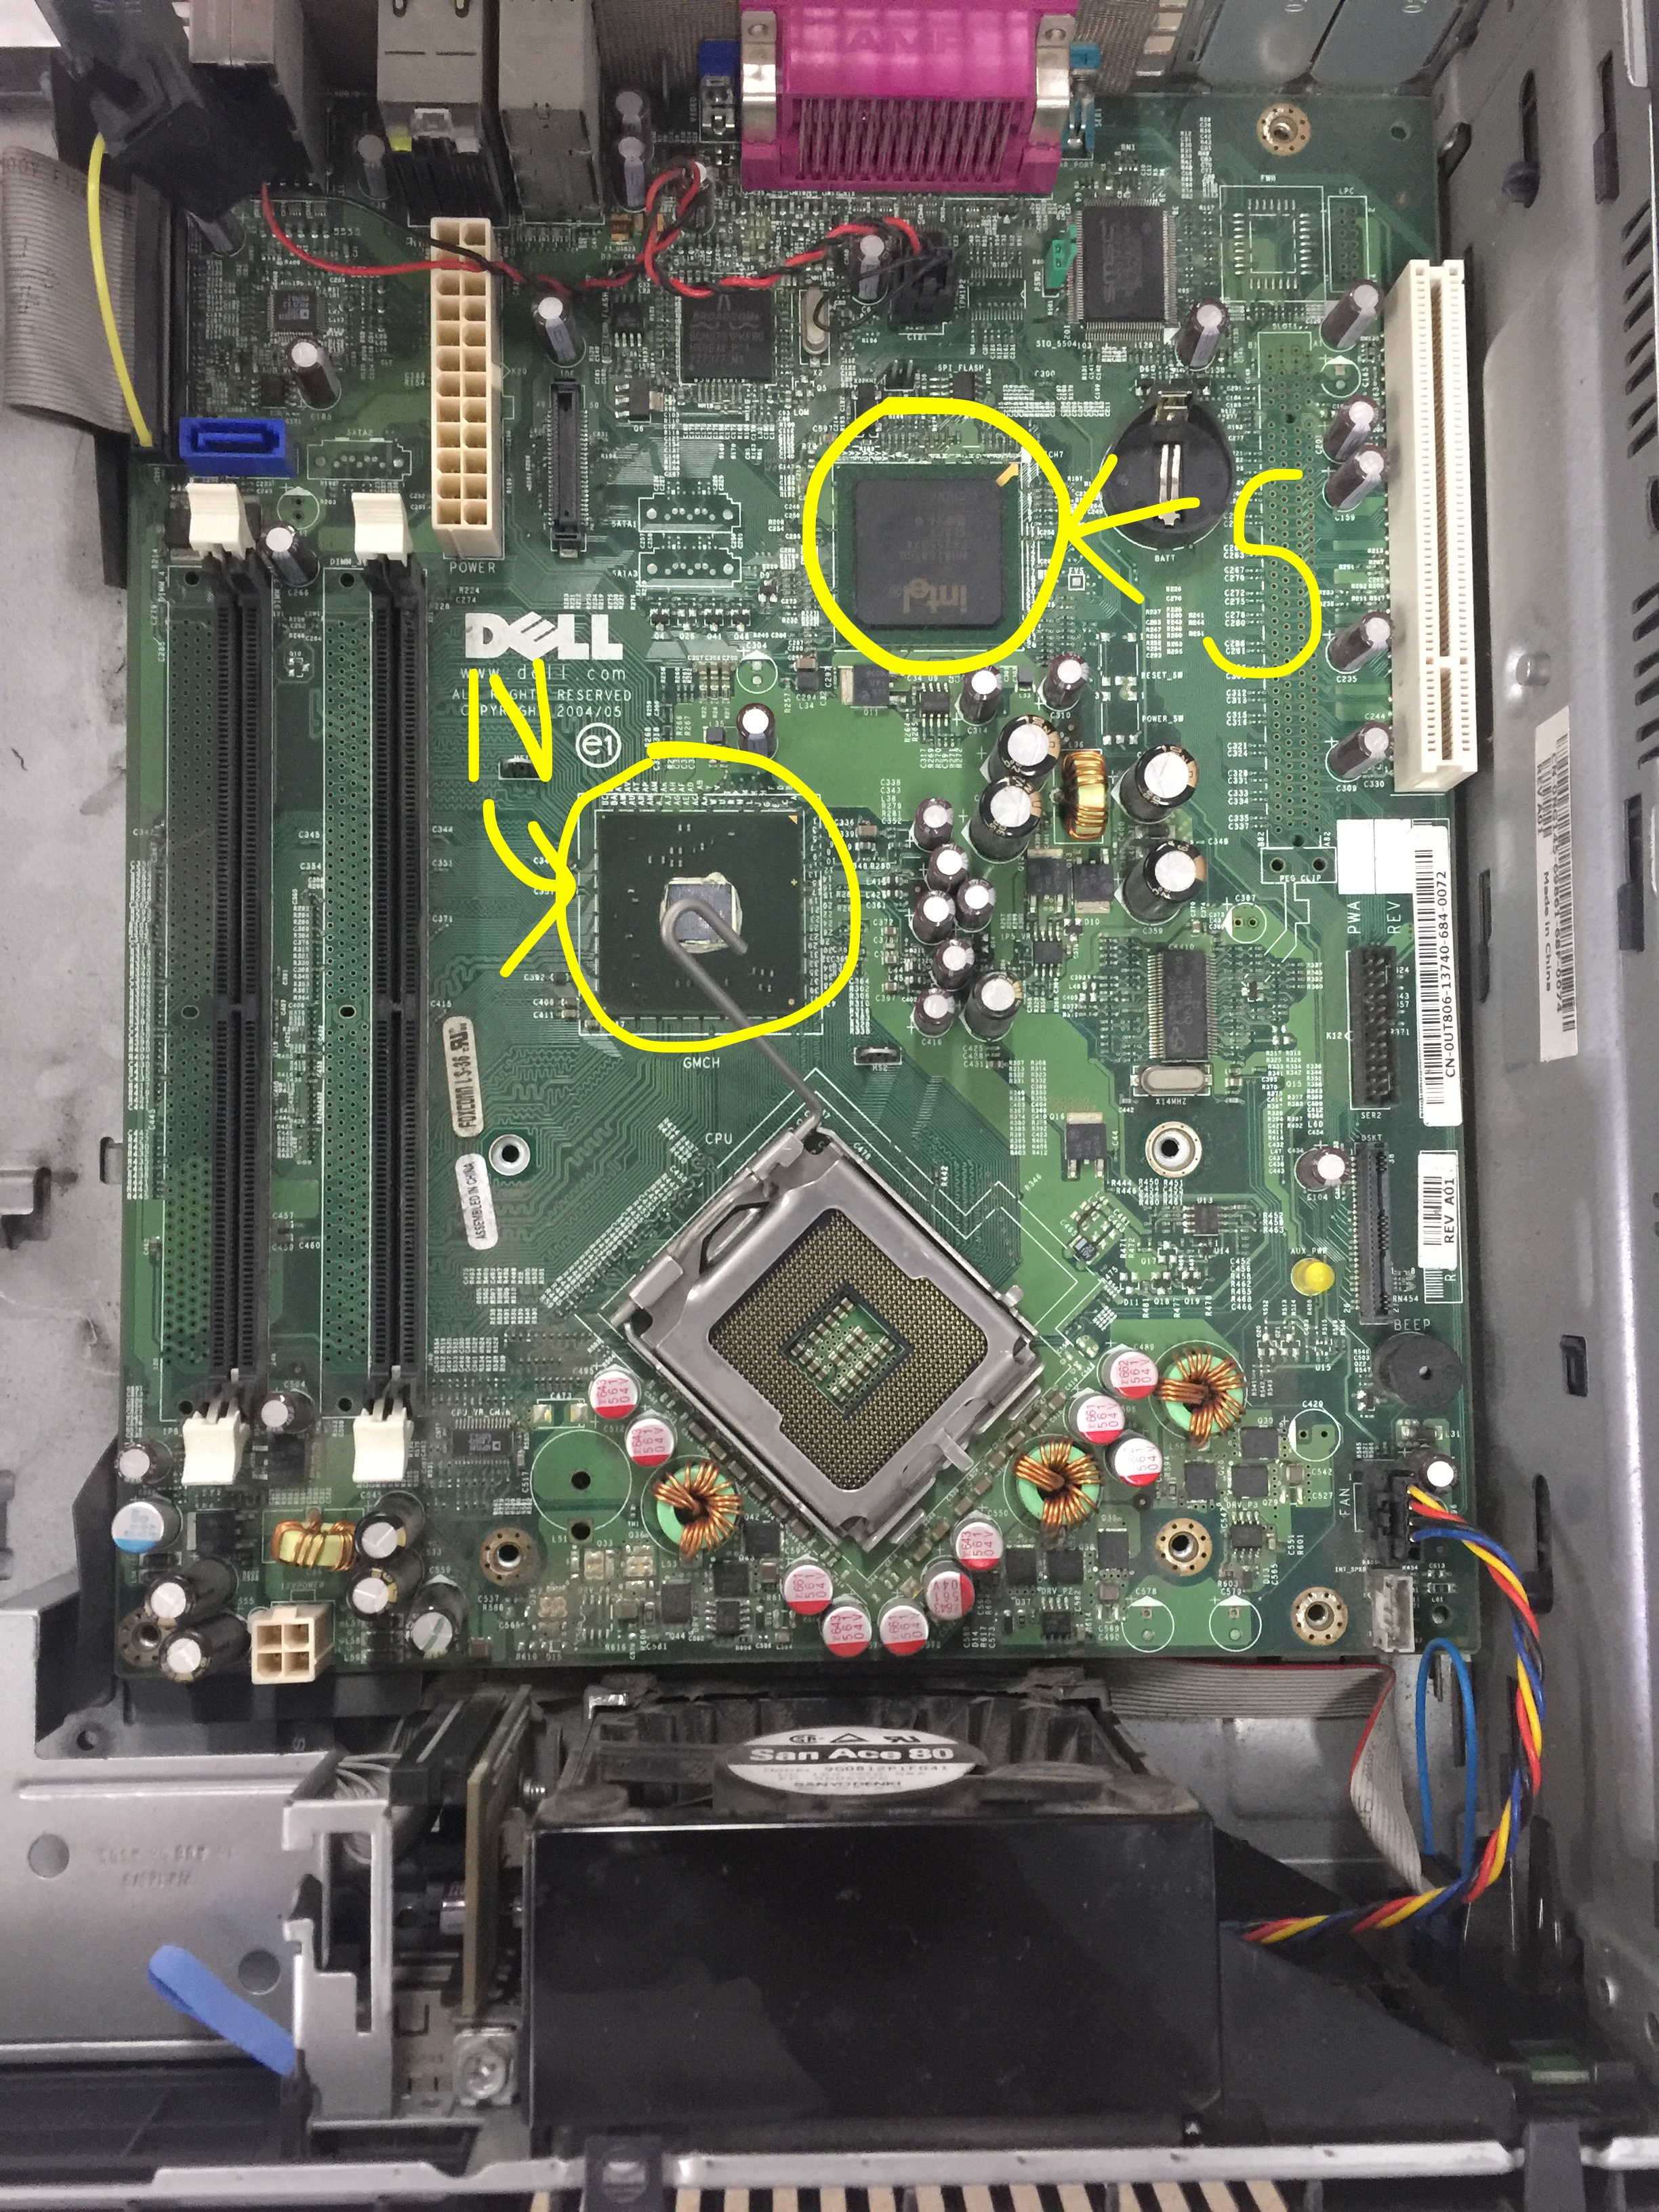
\includegraphics[scale=0.06]{bridge.jpg}
	\caption{The location of north bridge and south bridge on the mother board.}
	\end{center}
	\end{figure}
	\item \textbf{How are the North and South bridges connected together?}\\
	They are connected through internal bus.
	\item \textbf{What is the BIOS?}\\
	BIOS stands for Basic Input Output System.\\
	It is a program stored in the ROM, reserving the most basic functions of a computer, such as inputting, outputting and self-examining after the computer is turned on.
	\item \textbf{Take out the CPU, rotate it and try to plug it back in a different position, is that working?}\\
	No. There is a unique shape in one direction of the CPU, indicating the correct direction to insert.
	\item \textbf{Explain what overclocking is?}\\
	Overclocking is configuration of computer hardware components to operate faster than certified by the original manufacturer, with "faster" specified as clock frequency in megahertz.
	\item \textbf{What are pins on a PCI/PCI-e card and what are they used for?}\\
	\begin{figure}[h!]
	\begin{center}
	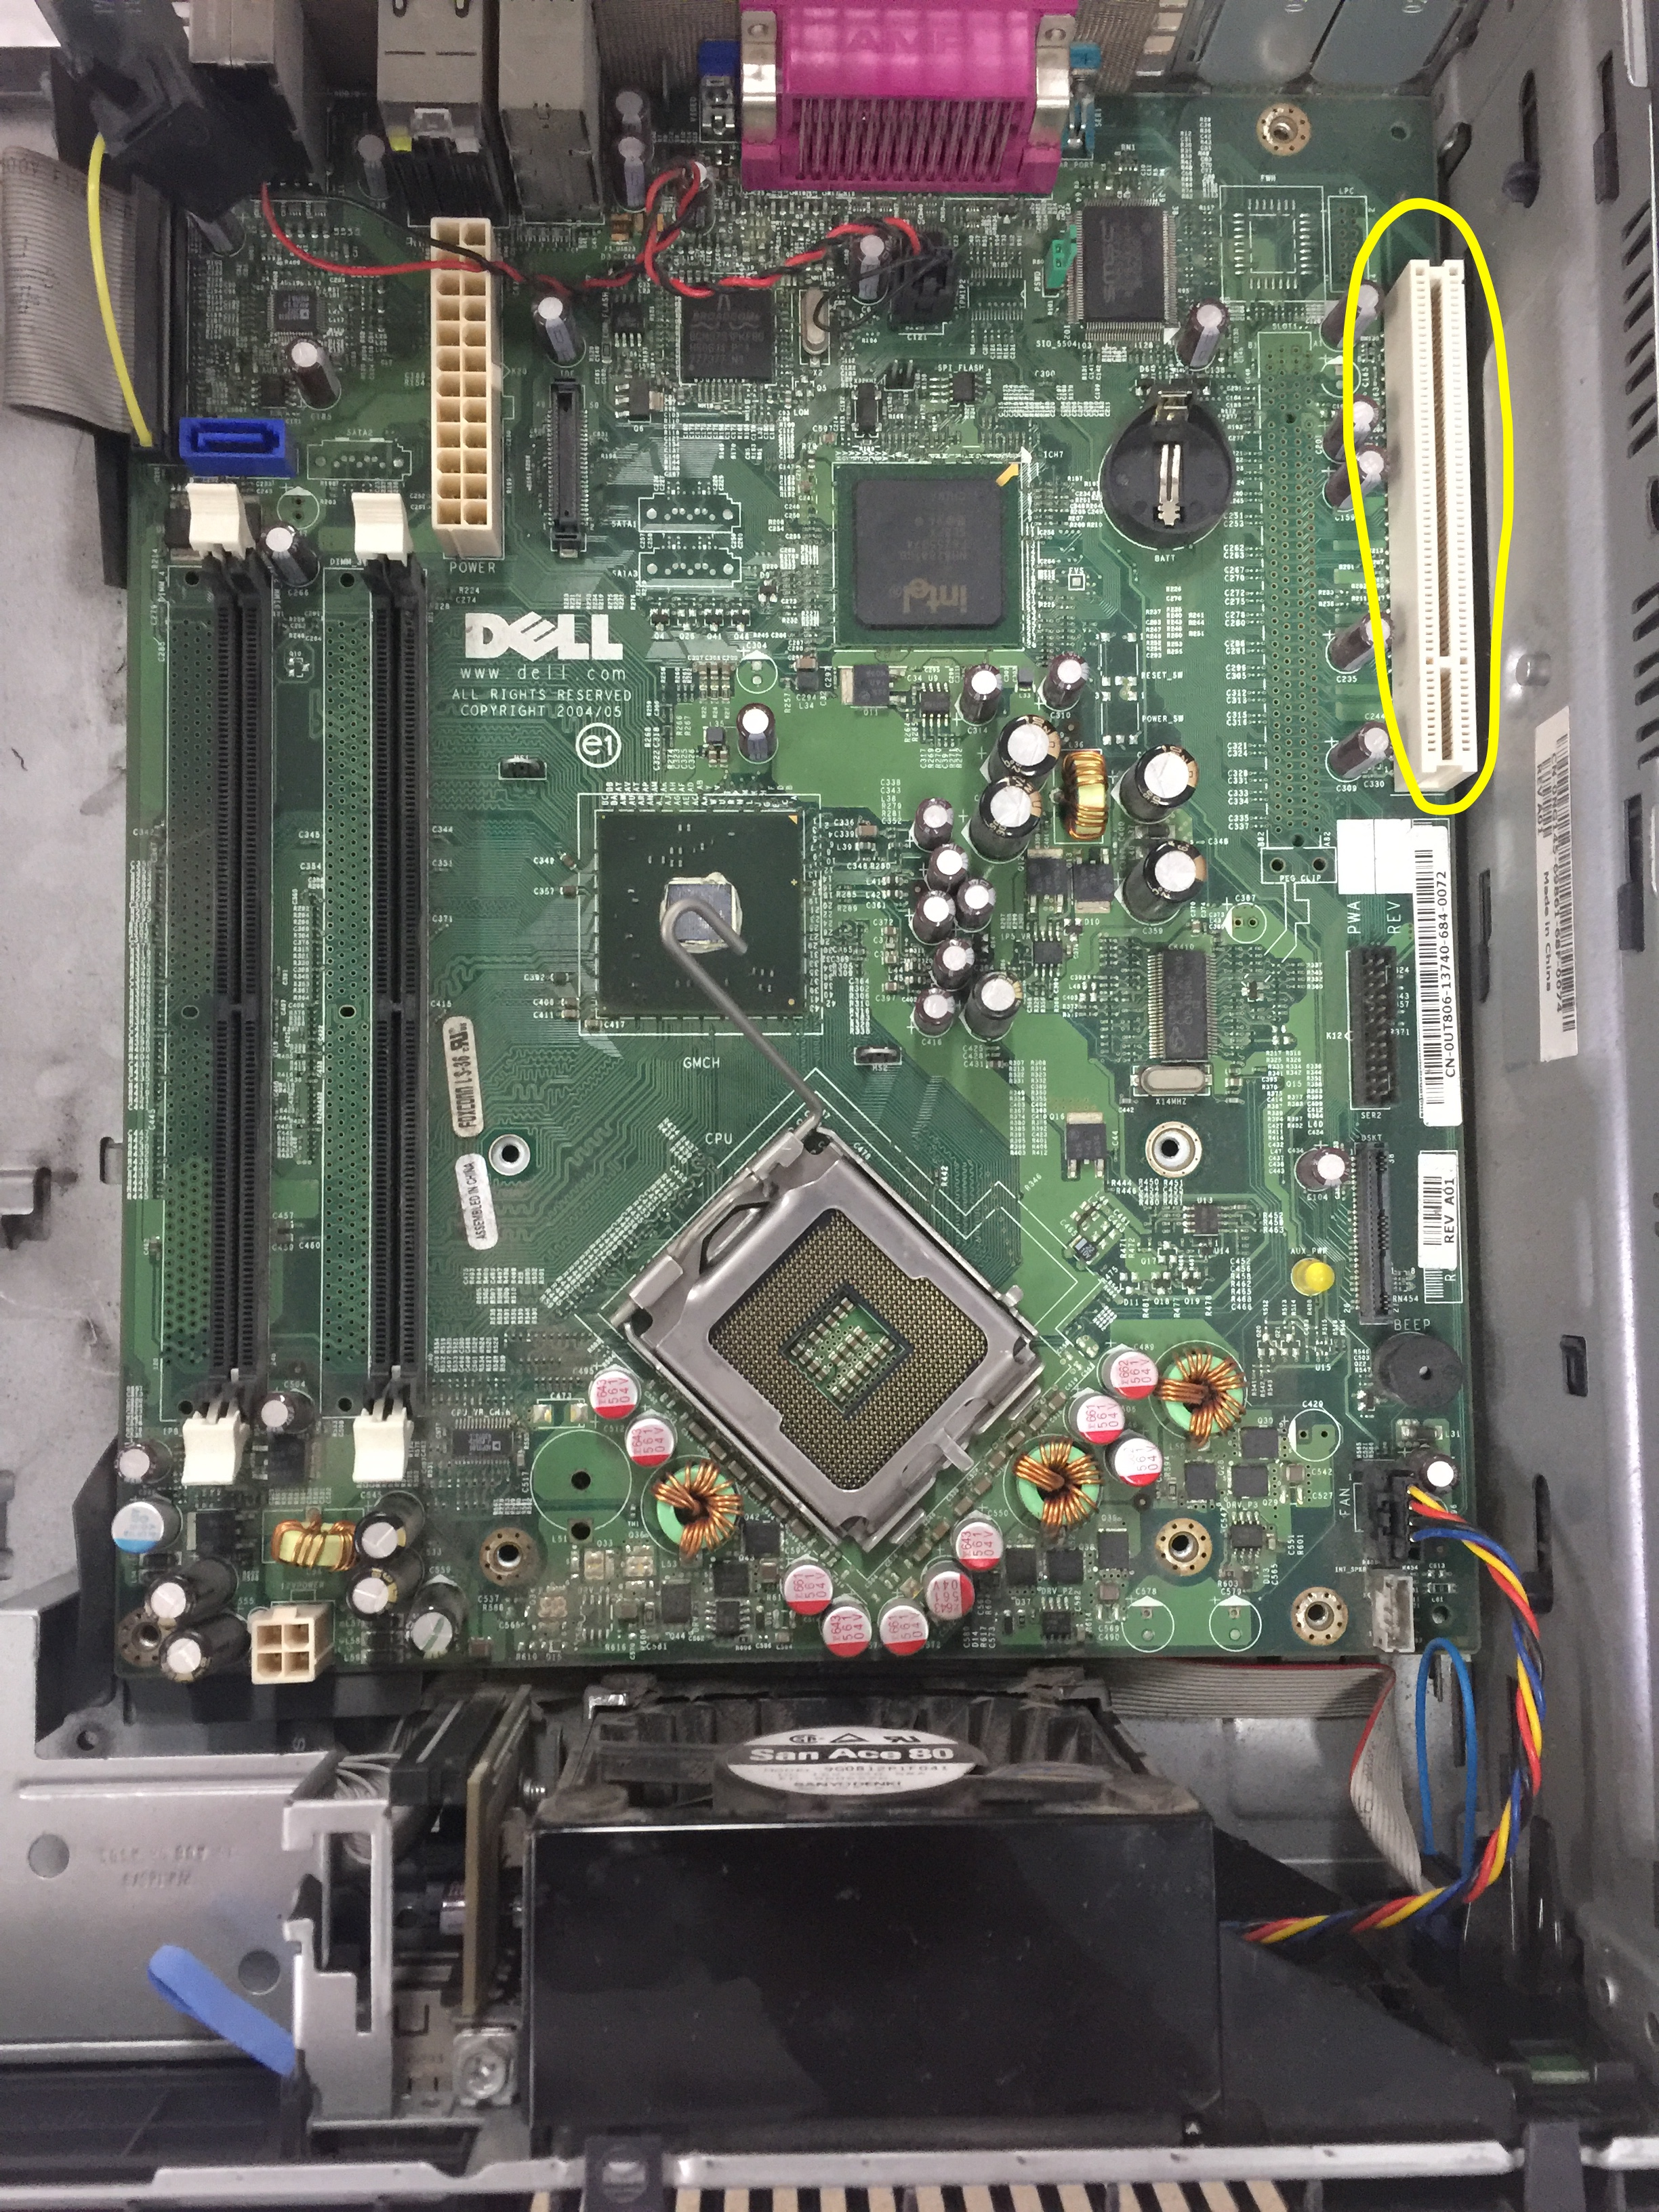
\includegraphics[scale=0.06]{PCI.jpg}
	\caption{The location of PCI on the mother board.}
	\end{center}
	\end{figure}
	Pins are the metal stuff shown in figure 3.\\
	They are used for communication between the motherboard and the PCI card.
	\item \textbf{Before PCI-e became a common standard many graphics cards were using Accelerated Graphics Port (AGP), explain why.}\\
	Because AGP uses a direct connection to the processor instead of sharing the PCI, thus reaching a higher processing speed.\\
	However, PCI-e performs even better than AGP. Therefore, PCI-e gradually becomes popular.
\end{itemize}
\end{document}